% CAMERA-READY version (PLAN 4.3). Same sections and tables as main.tex; the real author block
% and the acknowledgements live only here. Build with ./build.sh (writes build/main_camera.pdf).
% Paper: "Beating the Floor: A Leakage-Audited Benchmark of Recall Prediction for Spaced Repetition"
% Template: official EDM LaTeX template (edm_article.cls), from
%   https://educationaldatamining.org/wp-content/uploads/2024/EDM-template2024.zip
%   (linked from https://educationaldatamining.org/edm2026/instructions-for-authors/).
%   Copy kept in template_src/. Build with ./build.sh (TEXINPUTS points at template_src/).
% main.tex is the double-blind submission; this file is not submitted anonymously.
\documentclass{edm_article}

\usepackage{amsmath,amssymb}
\usepackage{booktabs}
\usepackage{graphicx}
\usepackage{url}

% Camera-ready switch. On here (camera-ready); main.tex sets it off (anonymous submission).
\newif\ifcamera
\cameratrue

\title{Beating the Floor: A Leakage-Audited Benchmark of Recall Prediction for Spaced Repetition}

% ORDER TBD by authors
\numberofauthors{5}
\author{
\alignauthor
Amal Verma\\
\affaddr{Veermata Jijabai Technological Institute (VJTI)}\\
\affaddr{Mumbai, India}\\
\email{\texttt{TBD}}
\alignauthor
Vedaang Pagnis\\
\affaddr{Veermata Jijabai Technological Institute (VJTI)}\\
\affaddr{Mumbai, India}\\
\email{\texttt{TBD}}
\alignauthor
Prathamesh Sankhe\\
\affaddr{Veermata Jijabai Technological Institute (VJTI)}\\
\affaddr{Mumbai, India}\\
\email{\texttt{TBD}}
\and
\alignauthor
Vaishvi Khandelwal\\
\affaddr{Veermata Jijabai Technological Institute (VJTI)}\\
\affaddr{Mumbai, India}\\
\email{\texttt{TBD}}
\alignauthor
[Supervisor name TBD]\\
\affaddr{Veermata Jijabai Technological Institute (VJTI)}\\
\affaddr{Mumbai, India}\\
\email{\texttt{TBD}}
}

\begin{document}

\maketitle

\begin{abstract}
Recall predictors for spaced repetition are usually compared with each other, rarely with a floor.
% PROTOCOL: 100 Anki users and all Duolingo users (EVALUATION.md 2). Not a result.
We compare them with constant-recall floors on two datasets: 100 Anki users and all Duolingo users.
We use one-step-ahead prediction, user-clustered bootstrap intervals and a same-session leakage audit.
On Duolingo, a constant (per user, smoothed) reaches a log loss of 0.2723.
% FACTS: Duolingo, Constant (per user, smoothed) log loss 0.2723
This beats FSRS-6 (opt.), at 0.3003, and half-life regression (HLR), at 0.4181.
% FACTS: Duolingo, FSRS-6 (optimised) log loss 0.3003; HLR (Settles & Meeder) log loss 0.4181
FSRS-6 (opt.) keeps default weights for 115,110 of 115,222 Duolingo users.
% FACTS: Duolingo, FSRS-6 (optimised) fallback to default weights: 115110 of 115222 users
On Duolingo, only gradient-boosted decision trees (GBDT) and Bayesian model v1 (Markov chain Monte Carlo, MCMC) beat the floor, v1 narrowly.
GBDT uses FSRS-state features and the learner's own history.
It beats FSRS-6 (opt.) on both datasets: on Anki the log-loss difference is $-$0.0210, with 95\% CI [$-$0.0284, $-$0.0144], and on Duolingo it is $-$0.0415.
% FACTS: Anki, GBDT minus FSRS-6 (optimised), log loss: diff -0.0210, 95% CI [-0.0284, -0.0144]. Duolingo, GBDT minus FSRS-6 (optimised), log loss: diff -0.0415
On srs-benchmark's public Anki protocol, GBDT beats FSRS-6 but trails RWKV-Instant.
Its Anki calibration gain over FSRS-6 is not significant.
Duolingo records each practice session at one timestamp, and a feature built from earlier rows can see outcomes from the same session.
Removing it changes the development-sample validation log loss of our first GBDT from 0.2473 to 0.2578.
% FACTS: Duolingo validation, frozen GBDT, log loss with the same-session leak: 0.2473; after the fix: 0.2578
Limits include an unconverged Bayesian decay parameter.
\end{abstract}

\keywords{spaced repetition, recall prediction, benchmark design, data leakage, gradient-boosted trees}

\section{Introduction}
Spaced-repetition schedulers decide when a learner should see an item again.
Each decision depends on a predicted probability of recall, so the quality of that predictor drives how much practice is wasted and how much is forgotten.
Recent work compares recall models with each other \cite{settles2016trainable, ye2022stochastic, srsbenchmark}.
A constant recall rate, fitted to training data only, is a floor that uses no memory model at all.
A floor is cheap, and it shows how much a model's structure adds.

We study this question on two datasets that differ a great deal.
Anki gives individually timed reviews of many cards.
Duolingo gives short practice sessions, many learners, and a high base rate of recall.
The two datasets differ in size and in scoring rule, so we report each one on its own terms.

The first result concerns the constant floor on Duolingo.
A smoothed per-user constant has log loss 0.2723.
FSRS-6 (optimised) has 0.3003, and half-life regression (HLR) has 0.4181.
% FACTS: Duolingo, Constant (per user, smoothed) log loss 0.2723; FSRS-6 (optimised) log loss 0.3003; HLR (Settles & Meeder) log loss 0.4181
Our maximum a posteriori (MAP) models v2 and v3 reach 0.2892 and 0.2830, so they also trail the constant.
% FACTS: Duolingo, Ours v2 log loss 0.2892; Ours v3 log loss 0.2830
The Bayesian model v1 reaches 0.2682, which is second only to GBDT, but it improves on the constant by only 0.0040.
% FACTS: Duolingo, Ours (GPU port) minus Constant (per user, smoothed), log loss: diff -0.0040
The v1 model is the same Bayesian family on both datasets: the original implementation on Anki and its GPU port on Duolingo.

The second result is a gradient-boosted decision tree model (GBDT) with features from the FSRS-6 state and from the learner's own history.
On Anki, GBDT has log loss 0.3584, against 0.3794 for FSRS-6 (optimised).
On Duolingo, it has 0.2588, against 0.3003.
% FACTS: Anki, GBDT log loss 0.3584; FSRS-6 (optimised) log loss 0.3794. Duolingo, GBDT log loss 0.2588; FSRS-6 (optimised) log loss 0.3003
On both datasets the log-loss difference is significant under a user-clustered paired bootstrap.
On Anki the difference is $-$0.0210, with 95\% CI [$-$0.0284, $-$0.0144].
On Duolingo it is $-$0.0415, with 95\% CI [$-$0.0423, $-$0.0406].
% FACTS: Anki, GBDT minus FSRS-6 (optimised), log loss: diff -0.0210, 95% CI [-0.0284, -0.0144]. Duolingo, GBDT minus FSRS-6 (optimised), log loss: diff -0.0415, 95% CI [-0.0423, -0.0406]
GBDT also has the lower Brier score and the higher AUC on both datasets.
% FACTS: Anki, GBDT minus FSRS-6 (optimised), Brier: diff -0.0059, 95% CI [-0.0082, -0.0041]; Anki, AUC: diff 0.0285, 95% CI [0.0185, 0.0402]; Duolingo, Brier: diff -0.0078; Duolingo, AUC: diff 0.1273
The Anki calibration difference is not significant, so we do not claim a calibration gain there.
% FACTS: Anki, GBDT minus FSRS-6 (optimised), ECE: diff -0.0042, 95% CI [-0.0132, 0.0012], CI includes 0
% TODO-SRSB: the srs-benchmark comparison of GBDT against RWKV, GRU and FSRS-6 is reported in Section 5; the GBDT numbers there are pending.

The third result is about the Bayesian model v1.
On Anki, v1 is worse than FSRS-6 (optimised), with a log-loss difference of 0.0427 and 95\% CI [0.0327, 0.0554].
% FACTS: Anki, Ours (dynamic, learned lambda) minus FSRS-6 (optimised), log loss: diff 0.0427, 95% CI [0.0327, 0.0554]
Its decay parameter $\lambda$ has not converged on either dataset: in the main runs the split R-hat is 2.44 on Anki and 2.48 on Duolingo, with effective sample sizes of 3.05 and 3.00.
% FACTS: v1 lambda, Anki: split R-hat 2.44, ESS 3.05. v1 lambda, Duolingo (GPU port): split R-hat 2.48, ESS 3.00
The predictions change little under two checks, but $\lambda$ must not be read as an estimate, so the v1 results on both datasets are provisional.
Section 5 treats the Bayesian model as a trade-off between interpretable, uncertainty-aware models and accurate predictors.

The fourth result is a same-session leakage pitfall in the Duolingo traces.
Duolingo records a whole practice session at one timestamp, so a feature built from earlier reviews can see outcomes from the same session.
On the Duolingo development sample, the frozen GBDT's validation log loss was 0.2473 with the leak and 0.2578 after the fix.
% FACTS: Duolingo validation, frozen GBDT, log loss with the same-session leak: 0.2473. Duolingo validation, frozen GBDT, log loss after the fix: 0.2578
We give the grouping rule that removes the leak.

In summary, we contribute:
\begin{itemize}
\item a comparison of recall predictors against constant floors, on two datasets, with one leakage-audited protocol and paired, user-clustered intervals;
\item evidence that a per-user constant beats FSRS-6 and HLR on Duolingo, and that GBDT beats FSRS-6 on both datasets;
\item the same-session leakage pitfall in Duolingo and how to avoid it;
\item a comparison of Bayesian (Markov chain Monte Carlo, MCMC, and MAP) and tree-based predictors, with their trade-offs.
\end{itemize}
Code will be released with the de-anonymised version.
% TODO: release link after review (anonymity).

Section 2 reviews related work.
Section 3 defines the data and the protocol.
Section 4 describes the models.
Section 5 reports the results, Section 6 discusses them, and Section 7 lists the limitations and disclosures.

\section{Related Work}
% TODO (3.3). Bullets from OUTLINE.md section 2:
% - Memory models: HLR (Settles & Meeder 2016), FSRS (Ye et al. 2022), ACT-R (Pavlik & Anderson 2005),
%   DAS3H (Choffin et al. 2019), Lindsey et al. 2014, KARL (Shu et al. 2024).
% - srs-benchmark: GRU, LSTM, RWKV; AVG and MOVING-AVG floors; MOVING-AVG beats FSRS-6 there.
% - GBDTs in neighbouring tasks: SLAM 2018 (Osika et al.; Settles et al.), knowledge tracing.
% - Benchmark hygiene and leakage (Kaufman et al. 2012).
% - Sources: paper/docs and the black book references.

\section{Data and Protocol}
% TODO (3.3). Bullets from OUTLINE.md section 3:
% - Anki: anki-revlogs-10k, 100 users, plus seeds 1 and 2 robustness samples.
% - Duolingo: Settles & Meeder traces, all users.
% - Event definition, per-user 80th-percentile time cutoff, one-step-ahead prediction, scored events.
% - Metrics: log loss, Brier, AUC, ECE, mean bias; user-clustered paired bootstrap.
% - Floors: global constant, per-user constant, smoothed per-user constant (m = 10, fixed in advance).
% - Leakage audit: figure or box on same-session timestamps and how they are grouped.

\section{Models}
% TODO (3.3). Bullets from OUTLINE.md section 4:
% - FSRS-6 (default and optimised), HLR, LagLogit.
% - v1: Bayesian dynamic retention model, Gibbs sampling with Polya-Gamma augmentation (GPU port).
% - v2 and v3: hierarchical FSRS-form models fitted by MAP.
% - GBDT (LightGBM): feature groups, frozen settings, validation-only selection.

\section{Results}
% TODO (3.4). Bullets from OUTLINE.md section 5:
% - Table 1: overall metrics on both datasets, floors at the top.
% - Table 2: paired differences vs FSRS-opt and vs smoothed constant, with user-win shares.
% - Figure: log loss by gap bin.
% - Figure: reliability diagrams.
% - Robustness: Anki seeds; GBDT overfitting checks (EVALUATION 12.1).
% - srs-benchmark (Phase 2): GBDT vs FSRS-6, RWKV, GRU, AVG, MOVING-AVG on held-out users.

% Tables and figures are generated by paper/scripts/ (do not edit the .tex tables by hand).
% Generated by paper/scripts/make_tables.py from paper/data/*_overall.csv. Do not edit.
\begin{table*}[t]
\centering
\caption{Overall metrics on Anki and Duolingo. Constants (top three rows) are floors: Const. global, Const. user, and Const. user (sm.), the per-user constant shrunk towards the global rate. FSRS-6 def. and opt. are FSRS-6 with default and optimised weights. v1 (MCMC) is the same Bayesian model on both datasets: the CPU MCMC on Anki and its GPU port on Duolingo. v2 and v3 are MAP fits. Bold: best non-constant model per column. Log loss (LL), Brier and ECE: lower is better; AUC: higher is better.}
\label{tab:overall}
\small
\setlength{\tabcolsep}{4pt}
\begin{tabular}{l rrrr rrrr}
\toprule
 & \multicolumn{4}{c}{Anki} & \multicolumn{4}{c}{Duolingo} \\
\cmidrule(lr){2-5}\cmidrule(lr){6-9}
Model & LL & Brier & AUC & ECE & LL & Brier & AUC & ECE \\
\midrule
Const. global (floor) & 0.454 & 0.141 & 0.500 & 0.004 & 0.279 & 0.074 & 0.500 & 0.003 \\
Const. user (floor) & 0.431 & 0.135 & 0.669 & 0.031 & 0.372 & 0.075 & 0.610 & 0.021 \\
Const. user (sm.) (floor) & 0.431 & 0.135 & 0.669 & 0.031 & 0.272 & 0.072 & 0.615 & 0.008 \\
\midrule
FSRS-6 def. & 0.396 & 0.121 & 0.745 & 0.012 & 0.302 & 0.078 & 0.566 & 0.051 \\
FSRS-6 opt. & 0.379 & 0.117 & 0.777 & 0.009 & 0.300 & 0.078 & 0.570 & 0.051 \\
HLR & 0.680 & 0.170 & 0.555 & 0.146 & 0.418 & 0.079 & 0.521 & 0.072 \\
LagLogit & not run & not run & not run & not run & 0.291 & 0.076 & 0.653 & 0.020 \\
v1 (MCMC) & 0.422 & 0.131 & 0.692 & 0.025 & 0.268 & 0.071 & 0.656 & 0.014 \\
v2 (MAP) & 0.379 & 0.117 & 0.778 & 0.013 & 0.289 & 0.075 & 0.609 & 0.035 \\
v3 (MAP) & 0.378 & 0.117 & 0.779 & 0.010 & 0.283 & 0.074 & 0.613 & 0.032 \\
GBDT & \textbf{0.358} & \textbf{0.111} & \textbf{0.805} & \textbf{0.005} & \textbf{0.259} & \textbf{0.070} & \textbf{0.697} & \textbf{0.001} \\
\bottomrule
\end{tabular}
\end{table*}


% Generated by paper/scripts/make_tables.py from paper/data/*_paired.csv and *_wins.csv. Do not edit.
\begin{table*}[t]
\centering
\caption{Paired log-loss differences (model minus reference; negative favours the model) with 95\% user-clustered bootstrap CIs, and the share of users whose log loss is lower for the model than for FSRS-6 (opt.). Reference: FSRS-6 (opt.) and the smoothed per-user constant.}
\label{tab:paired}
\small
\setlength{\tabcolsep}{4pt}
\resizebox{\textwidth}{!}{%
\begin{tabular}{l ccc ccc}
\toprule
 & \multicolumn{3}{c}{Anki} & \multicolumn{3}{c}{Duolingo} \\
\cmidrule(lr){2-4}\cmidrule(lr){5-7}
Model & vs FSRS-6 opt. & vs const. sm. & user win & vs FSRS-6 opt. & vs const. sm. & user win \\
\midrule
v1 (MCMC) & +0.043 [+0.033, +0.055] & $-$0.009 [$-$0.014, $-$0.004] & 22\% & $-$0.032 [$-$0.033, $-$0.031] & $-$0.004 [$-$0.004, $-$0.004] & 74\% \\
v3 (MAP) & $-$0.001 [$-$0.004, +0.002] & $-$0.053 [$-$0.067, $-$0.041] & 58\% & $-$0.017 [$-$0.018, $-$0.016] & +0.011 [+0.010, +0.011] & 72\% \\
GBDT & $-$0.021 [$-$0.028, $-$0.014] & $-$0.072 [$-$0.089, $-$0.058] & 82\% & $-$0.042 [$-$0.042, $-$0.041] & $-$0.013 [$-$0.014, $-$0.013] & 78\% \\
FSRS-6 opt. & -- & $-$0.051 [$-$0.067, $-$0.039] & -- & -- & +0.028 [+0.027, +0.029] & -- \\
\bottomrule
\end{tabular}}
\end{table*}


\begin{figure}[t]
\centering
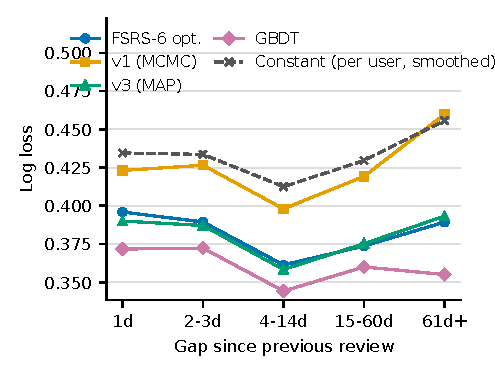
\includegraphics[width=\columnwidth]{figures/gaps_anki}
\caption{Caption TODO: log loss by gap bin, Anki.}
\label{fig:gaps-anki}
\end{figure}

\begin{figure}[t]
\centering
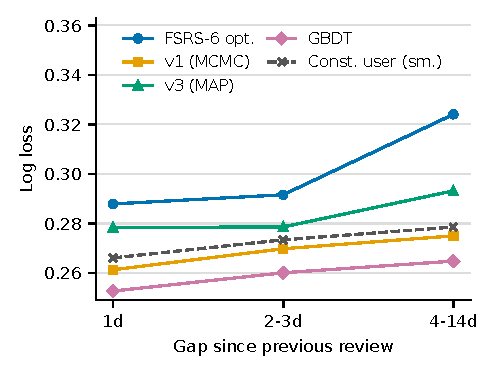
\includegraphics[width=\columnwidth]{figures/gaps_duolingo}
\caption{Caption TODO: log loss by gap bin, Duolingo.}
\label{fig:gaps-duolingo}
\end{figure}

\begin{figure}[t]
\centering
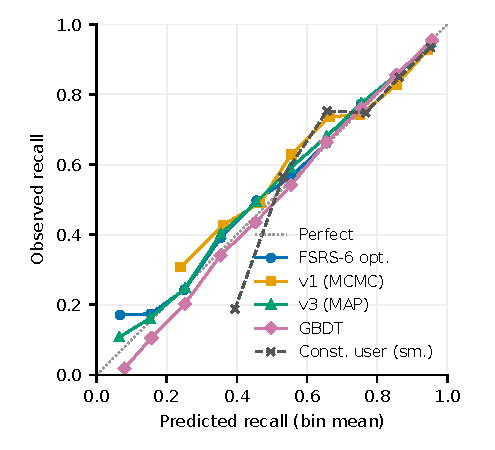
\includegraphics[width=\columnwidth]{figures/reliability_anki}
\caption{Caption TODO: reliability diagram, Anki. Bins with fewer than 30 reviews are omitted.}
\label{fig:rel-anki}
\end{figure}

\begin{figure}[t]
\centering
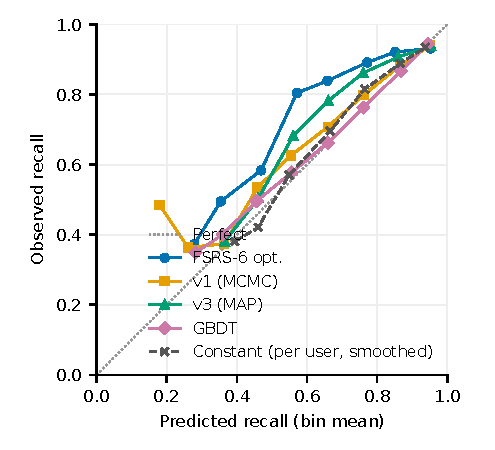
\includegraphics[width=\columnwidth]{figures/reliability_duolingo}
\caption{Caption TODO: reliability diagram, Duolingo. Bins with fewer than 30 reviews are omitted.}
\label{fig:rel-duolingo}
\end{figure}

% Generated by paper/scripts/make_tables.py from paper/data/anki_seeds*.csv. Do not edit.
\begin{table*}[t]
\centering
\caption{Anki robustness: log loss on three 100-user samples (seeds 0, 1, 2). The GBDT row gives the per-seed difference GBDT minus FSRS-6 (opt.) with its 95\% CI. v1 and v2 are not part of the robustness runs.}
\label{tab:seeds}
\small
\setlength{\tabcolsep}{3pt}
\begin{tabular}{l rrr r}
\toprule
Model & Seed 0 & Seed 1 & Seed 2 & Mean \\
\midrule
Const. global & 0.454 & 0.393 & 0.433 & 0.427 \\
Const. user & 0.431 & 0.361 & 0.406 & 0.399 \\
FSRS-6 def. & 0.396 & 0.325 & 0.364 & 0.362 \\
FSRS-6 opt. & 0.379 & 0.314 & 0.352 & 0.349 \\
HLR & 0.680 & 0.555 & 0.595 & 0.610 \\
v3 (MAP) & 0.378 & 0.308 & 0.351 & 0.346 \\
GBDT & 0.358 & 0.292 & 0.331 & 0.327 \\
\midrule
GBDT $-$ FSRS-6 opt. & $-$0.021 [$-$0.028, $-$0.014] & $-$0.023 [$-$0.037, $-$0.014] & $-$0.021 [$-$0.033, $-$0.012] & $-$0.022 \\
\bottomrule
\end{tabular}
\end{table*}


\section{Discussion}
% TODO (3.4). Bullets from OUTLINE.md section 6:
% - Why constants are strong on Duolingo: high base rate, short gaps, lexeme effects.
% - The ranking flips between datasets.
% - Bayesian vs ML trade-off: interpretability and uncertainty vs accuracy.
% - GBDT has no memory state, so it is a predictor, not a scheduler; a hybrid is future work.

\section{Limitations and Disclosures}
% TODO (3.4). Bullets from OUTLINE.md section 7:
% - Every item in EVALUATION.md 11.4 (a)-(i) must appear here.
% - One split; Anki sample size; v1 lambda does not converge; MAP fits;
%   FSRS-opt falls back to defaults on most Duolingo users; no scheduling simulation.

\section{Conclusion}
A constant recall rate is a strong floor on Duolingo, and most of the models we tested do not beat it there.
GBDT, a tree model with FSRS-state features and the learner's own history, beats FSRS-6 (optimised) on both datasets in log loss, and its Brier score is lower on both.
On Duolingo, FSRS-6 (optimised) keeps default weights for almost every user, so it is close to the default model. The Bayesian model v1 is the second best model on Duolingo, but its decay parameter has not converged, and it does not beat FSRS-6 on Anki.
Rankings change between datasets, so a benchmark needs both datasets and a floor.
The same-session leak in the Duolingo traces is a pitfall that any session-based benchmark should check for.


% Acknowledgements placeholder (EDM allows them in the camera-ready version only).
\section{Acknowledgments}
TBD: acknowledgements (funding, supervision, data access) to be written by the authors.

\bibliographystyle{abbrv}
\bibliography{references}

\end{document}
